\chapter{Cronograma}
\thispagestyle{fancy}
\section{Calendario de Actividades}
\noindent Para mostrar la delimitación de actividades usamos diagramas de Gantt, este diagrama nos permitira mostrar un flujo ordenado y esperado para el desarrollo de las actividades.
El proyecto se plantea desarrollar en 3 etapas antes ya mencionadas en los objetivos especificos \ref{sec:objetivos_especificos}(PT1, PT2, PT3), cada una de estas muestran las principales actividades, los principales objetivos a cumplir para cada etapa y por ultimo el tiempo esperado en el que se propone cumplir, vease en la figura\ref{fig:Diagrama_de_Actividades}:

\vspace{1cm}

\noindent Para delimitar los tiempos de cada actividad nos basamos en la metodologia ágil de \textit{Scrum}, en la que separamos por semanas las actividades refiriendonos a estas como \textit{sprints} o duración del sprint y al finalizar cada sprint se marca un perido de entrega y revision en esta hacemos referencia a la retrospectiva dentro de \textit{Scrum} como podemos observar en la figura \ref{fig:Diagrama_de_Actividades}

\vspace{1cm}
\noindent Seguir esta metodologia nos permitira defirnir tiempos de entrega ordenados siguiendo una secuencia y dando prioridad a el cumplimiento de cada objetivo secuencialemente de igual manera permitira manternos organizados y con revisiones constantes.

\begin{figure}
    \centering
    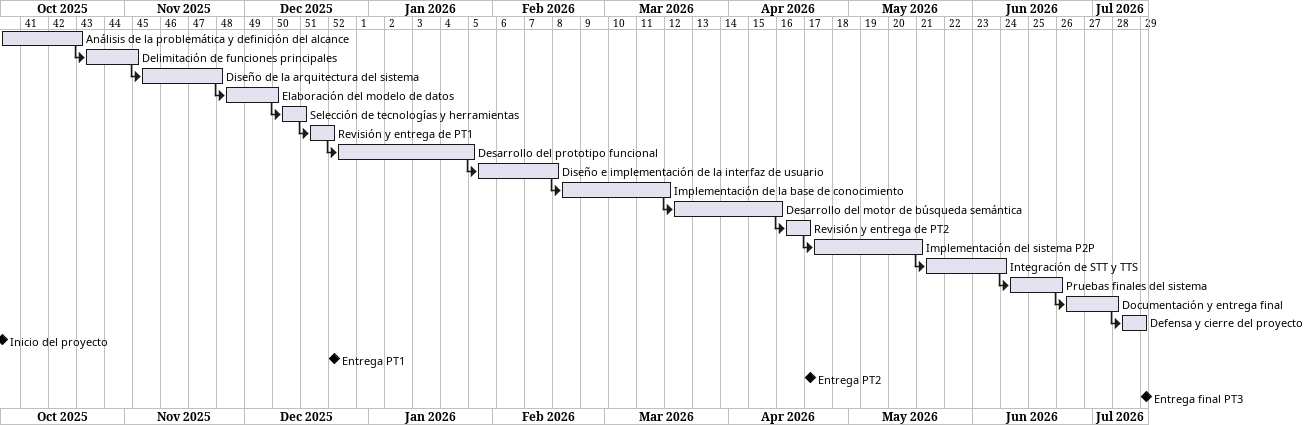
\includegraphics[angle=90, width=.4\linewidth]{diagramas/Calendario_Actividades_Gantt.png}
    \caption{Calendario de Actividades}
    \label{fig:Diagrama_de_Actividades}
\end{figure}